\chapter{Optimization}\label{section:optimization}

With the theoretical and pratical foundations of the model of farm/turbine power established, the following section treats the embedding of the trained model(s)  into a deterministic/stochastic optimization problem. The underlying theory of optimization under uncertainty and constraint learning is introduced before the actual optimization problems for the two turbine optimization problem are defined, the required models trained, and the results discussed.


\section{Optimization under Uncertainty}

Like in many areas, knowledge about the uncertainty associated with certain variables can change decisions in which these variables underlying uncertainty plays a part. For example, while optimizing anything from next year's crop to tomorrow's energy pricing, the field of Stochastic Programming is occupied with finding methods that allow for introducing these uncertainties into optimization problems.

One way to approach these uncertainties is to split the problem into scenarios. A bakery, for example, has to decide on how many Baguettes to bake for the next day to maximize its profit. Baking too few Baguettes will lead to missing out on potential sales, while baking too many baguettes will mean that the demand is fulfilled, but the money invested in the excess number of baguettes is lost. Assuming the mean number of baguettes bought every day is $1000$, the price to buy a baguette is $1 €$ and the cost to produce a baguette is $0,2 €$ the classical approach to solving such a problem would be by the following formulation \footnote{$x$ of course non-negative}: 


\begin{align*}
	\max_{x} \quad \left( 1.00 \cdot \min(x,1000) - 0.20 \cdot x \right)
\end{align*}


To represent uncertainty, additional scenarios of the demand being $10\%$ lower ($900$ Baguettes) and $10\%$ higher ($1100$ Baguettes) can be added. Assuming that the mean demand has a $50\%$ probability of occurring, the $10\%$ demand increases a $20\%$ probability and the $10\%$ decrease a $30\%$  probability, the problem can be modified to maximize the expected profit across these three scenarios by the formulation

\begin{align*}
	\max_{x} \quad & 0.5 \cdot \left(1.00 \cdot \min(x,1000) - 0.20 \cdot x \right) \\
	&+ 0.3 \cdot \left(1.00 \cdot \min(x,900) - 0.20 \cdot x\right) \\
	&+ 0.2 \cdot \left(1.00 \cdot \min(x,1100) - 0.20 \cdot x\right)
\end{align*}

Assuming only these three scenarios are possible, the result from this optimization problem would be the Expected profit and how many Baguettes are the optimal number of Baguettes to yield the maximum Expected profit across all scenarios. This would be optimal assuming there is no more information about the next day's demand, meaning that by using this approach, the total profit over a long time would be maximal. In case there is more information regarding the next day's demand, the probabilities that give the weights in this optimization might shift, with one scenario potentially reaching probability $100\%$ if there were to be absolute certainty that the next day's demand would be, for example, $1100$ baguettes. As having such exact information is very rare, the best solution will be in most cases to maximize the profit Expectation. 

The obvious connection to conventional statistical analysis is that the demand is a random variable that can take multiple values, in this case, we assumed it to be a discrete random variable $Y$ with support ${900,1000,1100}$ even though in real-world applications the demand of baguettes will move somewhere between $[0,\infty]$. Finding the Expectation for such a discrete random variable can be done as 

\[
\mathbb{E}[X] = \sum_{i} x_i \cdot \mathbb{P}(X = x_i) = \sum_{i} x_i p_i
\]

or for continuous random variables  
 
\[
\mathbb{E}[X] = \int_{-\infty}^{\infty} x \cdot f_X(x) \, dx
\]

Using these two expressions, optimization problems can thus be formulated to optimize the Expectation of objective functions containing random variables. \cite{BirgeLouveauxStochasticProgramming}


\section{Constraint Learning} \label{sec:constraint_learning}

Constraint learning refers to introducing a model that has learned relationships between certain variables from data into an optimization problem. In the case of constraint learning, the model is more specifically introduced into an optimization problem as a set of constraints. As many real-life relationships are dificult to represent by a simple analytical function, introducing machine learning models to optimization problems opens up many new possibilities \cite{FAJEMISIN20241}.

In the case of Neural Networks, one way of introducing a Neural Network as a constraint into an optimization problem is by recognizing that when using the Rectifier Linear Unit (ReLu) Function as activation function with the (linear) sum of neuron bias and weighted inputs $\tilde{v}_i^\ell$ being the function argument


\begin{equation}
	v_i^\ell = \max(0, \tilde{v}_i^\ell) = \max(0,  b_i^\ell + \sum_j w_{ij}^\ell v_j^{\ell - 1})
\end{equation}


the function can be rewritten as the following constraints 

\begin{align}
	v_i^\ell &\geq \tilde{v}_i^\ell \\
	v_i^\ell &\leq \tilde{v}_i^\ell - M^{\text{low}}(1 - j_i) \\
	v_i^\ell &\leq M^{\text{up}} j_i
\end{align}

with $j_i \in \{0,1\}$ a integer variable such that

\begin{align}
	j_i =
	\begin{cases}
		0 & \text{if } \tilde{v}_i^\ell < 0 \\
		1 & \text{if } \tilde{v}_i^\ell > 0
	\end{cases}
\end{align}

This decomposition allows for introducing a Neural Network into an optimization problem by decomposing it into the shown set of mixed-integer linear constraints \cite{ALCANTARA2023120895}.

\section{The Two Turbine Problem}

Optimizing the positioning of two wind turbines can be expressed as optimizing the relative position of a second wind turbine $T_2$ to a fixed first turbine $T_1$, defined by the relative distances $\Delta x$ and  $\Delta y$. Both  $\Delta x$ and  $\Delta y$ are constrained by minimum distance $\Delta_{min}$ to  $T_2$ and maximum distances $\Delta x_{max}$/$\Delta y_{max}$ to make the problem bounded. 
This problem can be visualized as shown in Figure \ref{fig:two_turbine_problem}.

\begin{figure}[h] 
	\centering
	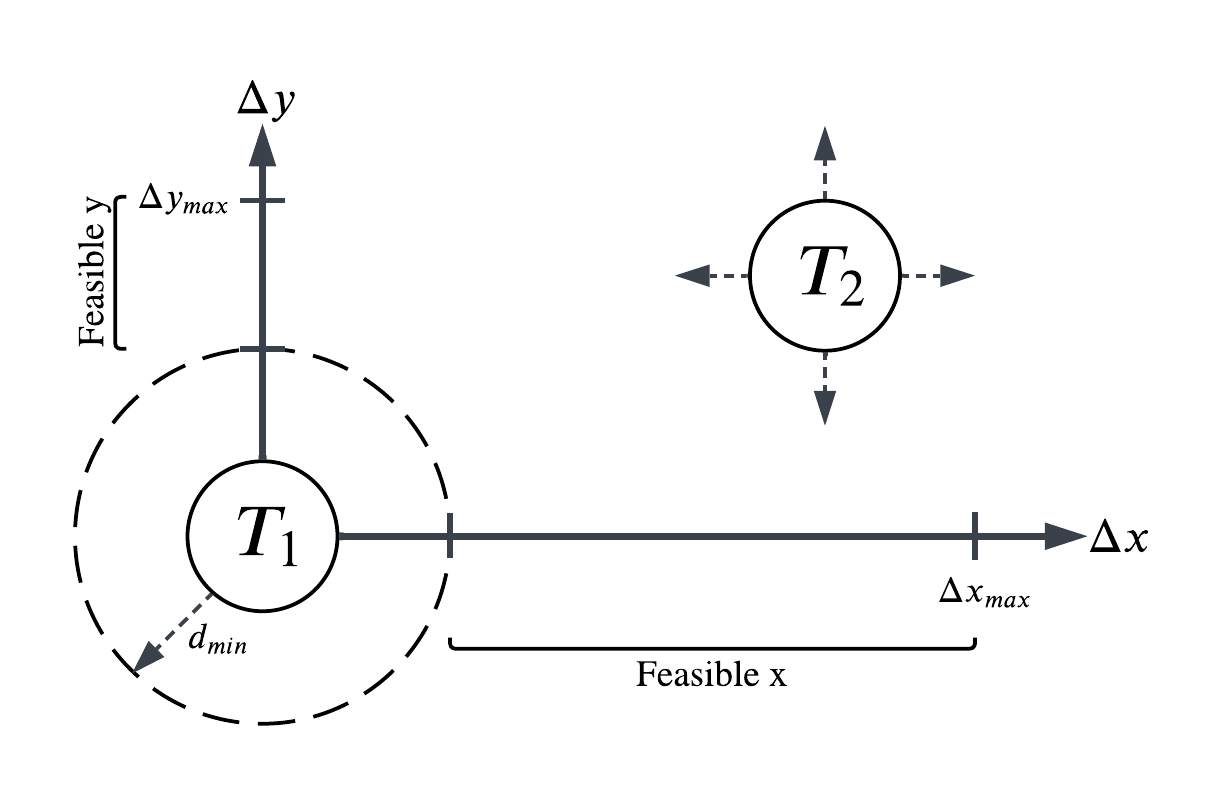
\includegraphics[width=0.6\textwidth]{figures/optimization/two_turbine_problem_schematic.png} % file name without extension
	\caption{Optimizing the relative position $\Delta x$/$\Delta y$ of a second wind turbine $T_2$ to a fixed first turbine $T_2$, constrained by minimum distance $d_{min}$ to  $T_1$ and maximum distances $\Delta x_{max}$/$\Delta y_{max}$}
	\label{fig:two_turbine_problem}
\end{figure}

The objective function to be optimized is the total power generation, e.g. the sum of power generated by both turbines. This objective is a function of both the position of the wind turbine as well as of the wind conditions like wind direction and wind speed. 

$$
f_{total Power}(x,y,\text{windspeed},\text{wind direction}, \text{(...)})
$$

Different from the geographic coordinates, the wind condition parameters like windspeed are inherently not deterministic and follow distributions like the normal distribution as shown in Figure \ref{fig:wind_dist}.

\begin{figure}[h] 
	\centering
	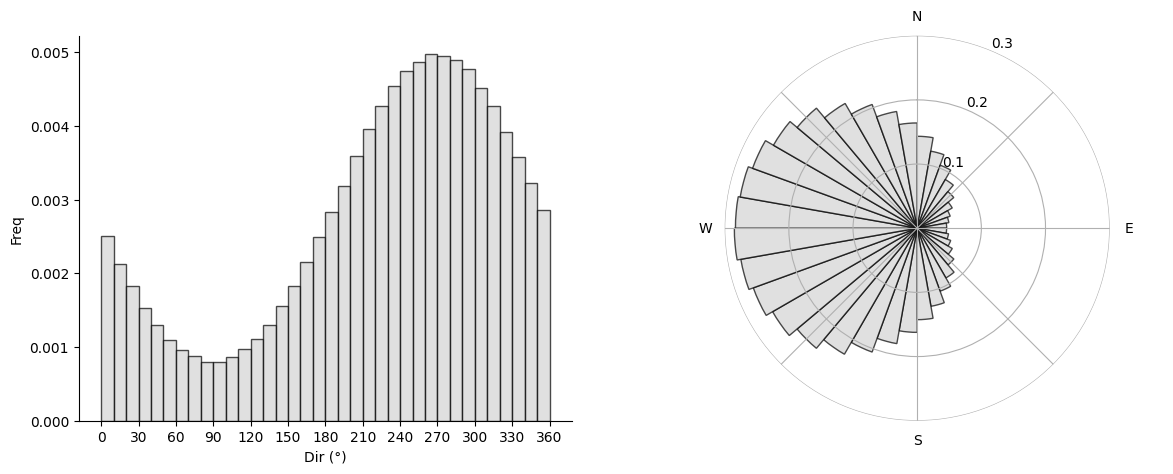
\includegraphics[width=0.9\textwidth]{figures/optimization/wind_dist.png} % file name without extension
	\caption{Histogram and Polar Plot across radiants for a normally distributed wind direction probability density function with mean West}
	\label{fig:wind_dist}
\end{figure}

The two main challenges of the optimization of the two-turbine problem are thus: 

\begin{enumerate}
	\item Introduce the complex relationship between turbine position, wind conditions, and power output into the optimization problem
	\item Introduce the non-deterministic nature of wind conditions into the optimization problem
\end{enumerate}

The first of these challenges is tackled by applying the Neural Network models discussed in Section \ref{sec:modelling} and introducing them into the optimization problem via constraint learning as described in Section \ref{sec:constraint_learning}. For the second problem, multiple approaches are now explored in the following subsections.


\subsection{Deterministic Optimization}

To begin solving the problem, the simplest approach is to assume the wind conditions to be discrete. In application, this might be analogous to using the Expectations of the joint probability distribution of all wind condition parameters, which in pratical terms would be considered the "principal wind direction". Taking these parameters as constant and homogeneous across the entire parameter space, the result is an objective function that is effectively only dependent on the relative positions of the turbine with the previously discussed geometrical constraints.

\begin{align}
	\max_{\mathbf{x}, \mathbf{y}} & f_{Power,\text{NN}}(\Delta x, \Delta y) \\
	\text{s.t.} \quad 
	&  0 \leq \Delta x \leq X_{\max} \\
	&  0 \leq \Delta y \leq Y_{\max} \\
	& \sqrt{(\Delta x)^2 + (\Delta y)^2} \geq d_{\min}
\end{align}

where:
\begin{itemize}
	\item \( (\Delta x, \Delta y) \) are the relative distances of the two turbines
	\item \( f_{Power, \text{NN}}(\Delta x, \Delta y)\) is a neural network (deterministic) approximating the total farm power output
	\item \(  X_{\max}, Y_{\max} \) define the maximal distance the two turbines can be placed apart
	\item \( d_{\min} \) is the minimum distance between the two turbines
\end{itemize}



The Notebook belonging to this formulation can be found in \href{https://github.com/schmeti/uc3m_TFM_wind_farm_optimization_codebase/blob/main/Windfarm_power_modelling/0_two_turbine_problem_constrLearn_determin.ipynb}{Deterministic Fomulation Notebook} \cite{schmetz2025twoturbine_determ}

\subsubsection{Modelling}

To begin with, the simulations to generate the dataset used to train the corresponding model for the deterministic case have to be generated. For the deterministic optimization, the position of the second turbine is variable in the given bounds and with an even steplength  as shown in Table \ref{tab:val_determ_data}. All remaining airflow characteristics remain constant (deterministic).

\begin{table}[ht]
	\centering
	\caption{Value Ranges for Deterministic Two Turbine Problem Data Set}
	\begin{tabular}{|l|c|c|c|}
		\hline
		\textbf{Variable} & \textbf{Const/Variable} & \textbf{Value} & Step Length\\
		\hline
		$\Delta x_{\text{turb2}}$ & Variable & [0, 5000] m & 50 m\\
		$\Delta y_{\text{turb2}}$ & Variable & [0, 500] m & 50 m \\
		wind\_speed & Constant & 8 m/s & -\\
		wind\_direction & Constant & 270°&- \\
		turbulence\_intensity & Constant & 0.06 & - \\
		\hline
	\end{tabular}

	\label{tab:val_determ_data}
\end{table}

In line with the parameter space defined in Table \ref{tab:val_determ_data}, simulations are performed as described in Section \ref{sec:model_pipe}. The resulting dataset is then introduced into the Neural Network optimization method, yielding Figure \ref{fig:determ_nn_opti}. When considering the results, it is apparent that models with a number of layers greater or equal than two and greater or equal than 8 nodes per hidden layer are nearly identical in performance. \textit{The chosen model configuration is therefore a $\text{NN}(5\,{-}\,8^{\times2}\,{-}\,1)$}, yielding good performance while reducing model size as much as possible, to be implemented in the optimization problem. 

\begin{figure}[h] 
	\centering
	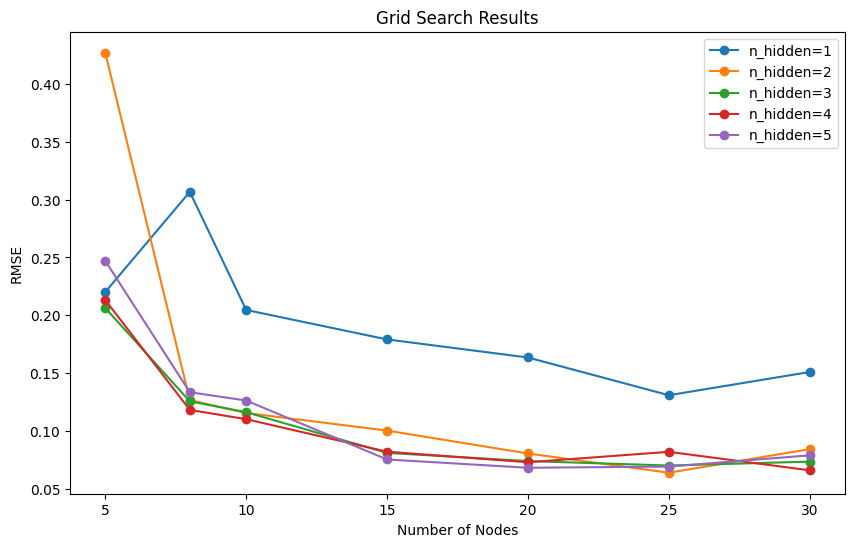
\includegraphics[width=0.7\textwidth]{figures/optimization/determ_nn_opti.png} 
	\caption{Grid search for Neural Network parameters for the deterministic model, showing how models with $n_{hidden} \geq 2$ and $n_{nodes} \geq 8$ yield near identical performance}
	\label{fig:determ_nn_opti}
\end{figure}

To validate the chosen model and gain a deeper understanding of its predictive power, we proceed to visualize the total power output across the variable parameter space. Figure \ref{fig:determ_model_colormap} shows a colormap generated from linealy interpolating between the datapoints for the simulation data (Subplot 1), a finer grid of predictions of the model (Subplot 2) and a colormap of the percentage deviation between model prediction and true simulation values (calculated at points and then again linearly interpolated). The color in the first two subplots represents the \textit{total power generated of both wind turbines}, with the second turbine placed at the given x/y location We find that the model appears to overall represents the behaviour well, with only systematic deviation occuring at locations very close to the first wind turbine at the origin. As the simulation allows for placing wind turbines at the exact same location and with corresponding results unrealistic, simulations in this area are not necessarily correct in results either. For the optimization, the minimum distance constraint removes this area from the feasible region, meaning that the comparatively large deviations there do not affect the optimization. 

\begin{figure}[h] 
	\centering
	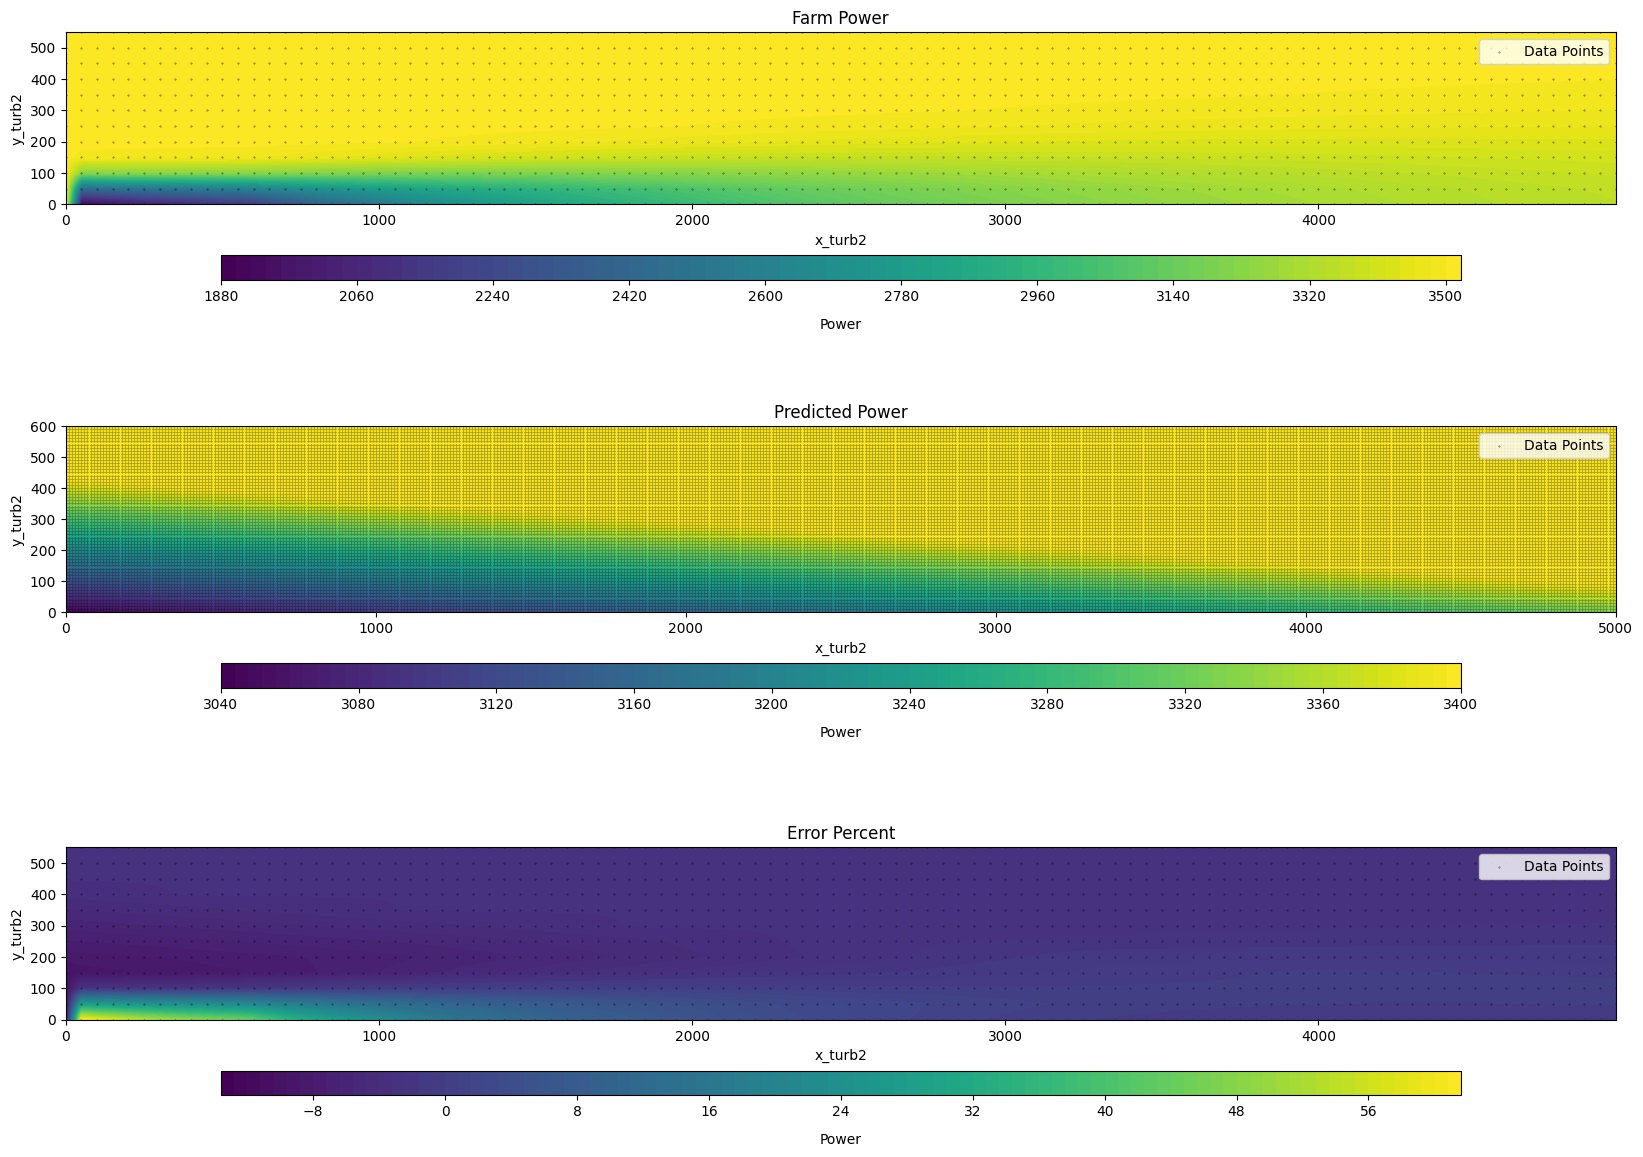
\includegraphics[width=1\textwidth]{figures/optimization/determ_model_colormap.png} 
	\caption{Colormap showing the Farm Power distribution for the second turbine being placed at any given x/y based on linear interpolation for real data, predicted data and the resulting percentage deviation, indicating overall good fit with only area of major deviation extremly close to turbine 1, an area excluded from the feasible region of the optimization problem }
	\label{fig:determ_model_colormap}
\end{figure}

The model thus appears to be suitable to represent the interactions between the two turbines and we proceed to the optimization.

\subsubsection{Optimization}


With the model trained and validated, we proceed to implementing the defined optimization problem in Pyomo  and embed the trained model using the approach described in Section \ref{sec:constraint_learning}.

When solving this problem as defined using Gurobi, a major challenge becomes apparent as the result shows that there is an large number of equally optimal solutions (e.g. degeneracy of the problem, see  \cite{vanderbei2020chapter3} for an exact definition of degeneracy) everywhere outside the wake of turbine 1, as can be seen  in the visualization of the optimization result found in \ref{fig:opti_determ270}.


\begin{figure}[h] 
	\centering
	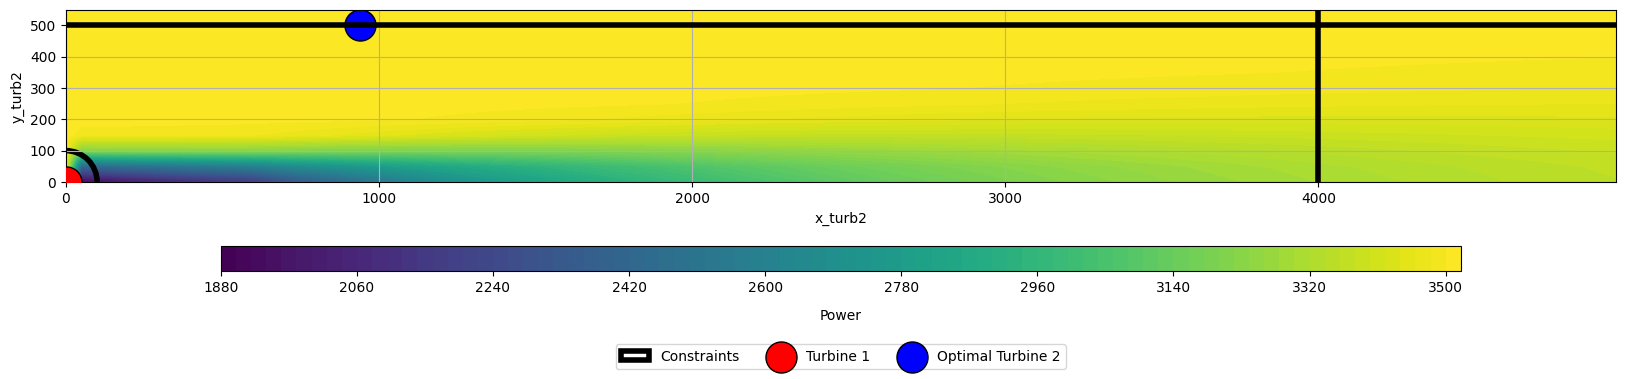
\includegraphics[width=1\textwidth]{figures/optimization/opti_determ270.png} 
	\caption{Deterministic optimization of the relative position of two wind turbines relative to each other with wind direction 270° and constant windspeed}
	\label{fig:opti_determ270}
\end{figure}

The existence of a large number of optimal values thus has to be taken into account moving forward.

\subsection{Stochastic Optimization} \label{sec:stoch_opti_1}

As the deterministic optimization does not account for the distribution of wind condition parameters and has found that the deterministic approach leaves a range of infinite global optima outside of the wake of turbine 1, the next step is to proceed with the introduction of uncertainty of the wind condition parameters into the problem. To do so, the objective function is modified to represent the expected power generated by the farm, if a turbine were to be placed at a given location. The Neural Network thus now has to be able to predict the power output for a given turbine 2 location, taking into account the wind condition parameters like direction and speed at a given location. The problem is formulated as follows: 

\begin{align}
	\max_{\mathbf{x}, \mathbf{y}} &  \sum_{i=1}^{n} f_{Power,\text{NN}}(\Delta x, \Delta y, \text{wind condition})\cdot p_{n,\text{wind condtion combination}} \\
	\text{s.t.} \quad 
	&  \Delta x \leq X_{\max} \\
	&  \Delta y \leq Y_{\max} \\
	& \sqrt{(\Delta x)^2 + (\Delta y)^2} \geq d_{\min}
\end{align}

Where:
\begin{itemize}
	\item \( (\Delta x, \Delta y) \) are the relative distances of the two turbines,
	\item \( f_{Power, \text{NN}}(\Delta x, \Delta y)\) is a deterministic neural network  approximating the total power output for turbine positions and wind conditions
	\item \(  X_{\max}, Y_{\max} \) define the maximal distance the two turbines can be placed apart
	\item \( d_{\min} \) is the minimum distance between the two turbines
	\item \(p_{n, \text{wind condtion combination}}\) is the probability corresponding to each of the scenarios
	\item \( n \) is the index of the discretized possible combinations of wind conditions 
\end{itemize}

The following section will first treat the univariate case of only wind direction being random, while wind speed and turbolence intensity remain constants. 


The Notebook belonging to this formulation can be found in \href{https://github.com/schmeti/uc3m_TFM_wind_farm_optimization_codebase/blob/main/Windfarm_power_modelling/0_two_turbine_problem_constrLearn_probweighted.ipynb}{Stochastic optimization with farm power NN Fomulation Notebook} \cite{schmetz2025twoturbine_stoch1}

\subsubsection{Modelling}

Like for the deterministic case, we begin by finding a fitting Neural Network model that can be embedded into the optimization problem. To do so, we again define the parameter space, this time with wind direction being variable and set up in a grid with step length of 10°. The full parameter grid is defined in Table \ref{tab:val_prob_data}

\begin{table}[ht]
	\centering
	\caption{Value Ranges for Probabilistic Two Turbine Problem Data Set}
	\begin{tabular}{|l|c|c|c|}
		\hline
		\textbf{Variable} & \textbf{Const/Variable} & \textbf{Value} & \textbf{$Steplength$}\\
		\hline
		$\Delta x_{\text{turb2}}$ & Variable & [0, 5000] m & 50 m\\
		$\Delta y_{\text{turb2}}$ & Variable & [0, 500] m  & 50 m\\
		wind\_speed & Constant & 8 m/s & -\\
		wind\_direction & Variable & [180°, 270°]& 10° \\
		turbulence\_intensity & Constant & 0.06 & - \\
		\hline
	\end{tabular}
	\label{tab:val_prob_data}
\end{table}

We then proceed to hyperparameter tuning of the model. Due to the added complexity, the model size has to be increased significantly to yield similarly good results compared to the deterministic case. As apparent in Figure \ref{fig:determ_nn_opti}, the performance appears to flatline for models with or more than 2 layers and with or more than 50 nodes, yielding similar performance. To minimize the number of nodes, we thus proceed with the initial model configuration $\text{NN}(5\,{-}\,50^{\times2}\,{-}\,1)$ for the following optimization.


\begin{figure}[h] 
	\centering
	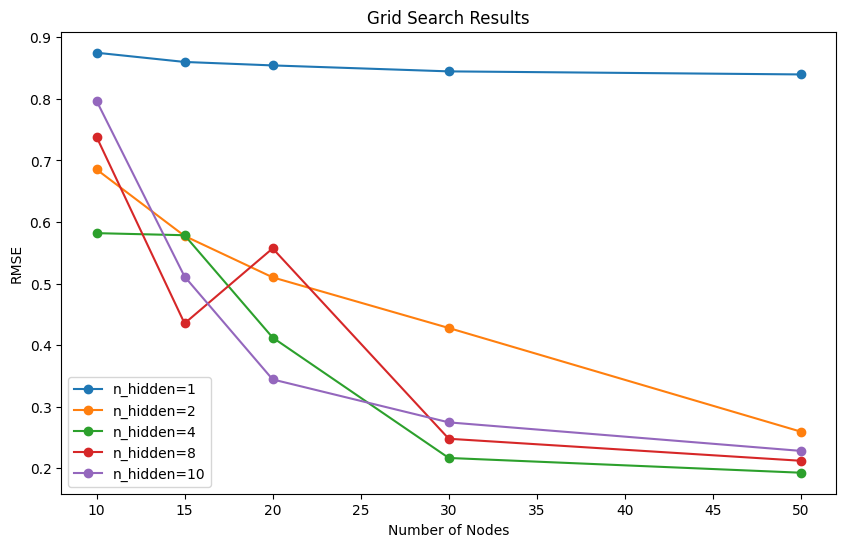
\includegraphics[width=0.62\textwidth]{figures/optimization/prob_nn_opti.png} 
	\caption{Grid Search results for a Neural Network configuration to predict for data with variable wind direction, showing similar performance for models of layers greater or equal than two, starting at 50 or more nodes}
	\label{fig:determ_nn_opti}
\end{figure}


With a model chosen, we again investigate its performance and find that even with the significantly more complex model, the results are not as good as for the model only trained for the deterministic case. While visually the shape of the wake generally appears to fit, the deviation in percent shows greater deviation, especially at greater distances away from Turbine 1 for the case of wind direction 260°, as shown in Figure \ref{fig:prob_model_colormap}. The model appears to also show some artifacts, with the most notable being the highest values in parallel to the wake right at the borders of the wake flow itself.

\begin{figure}[h] 
	\centering
	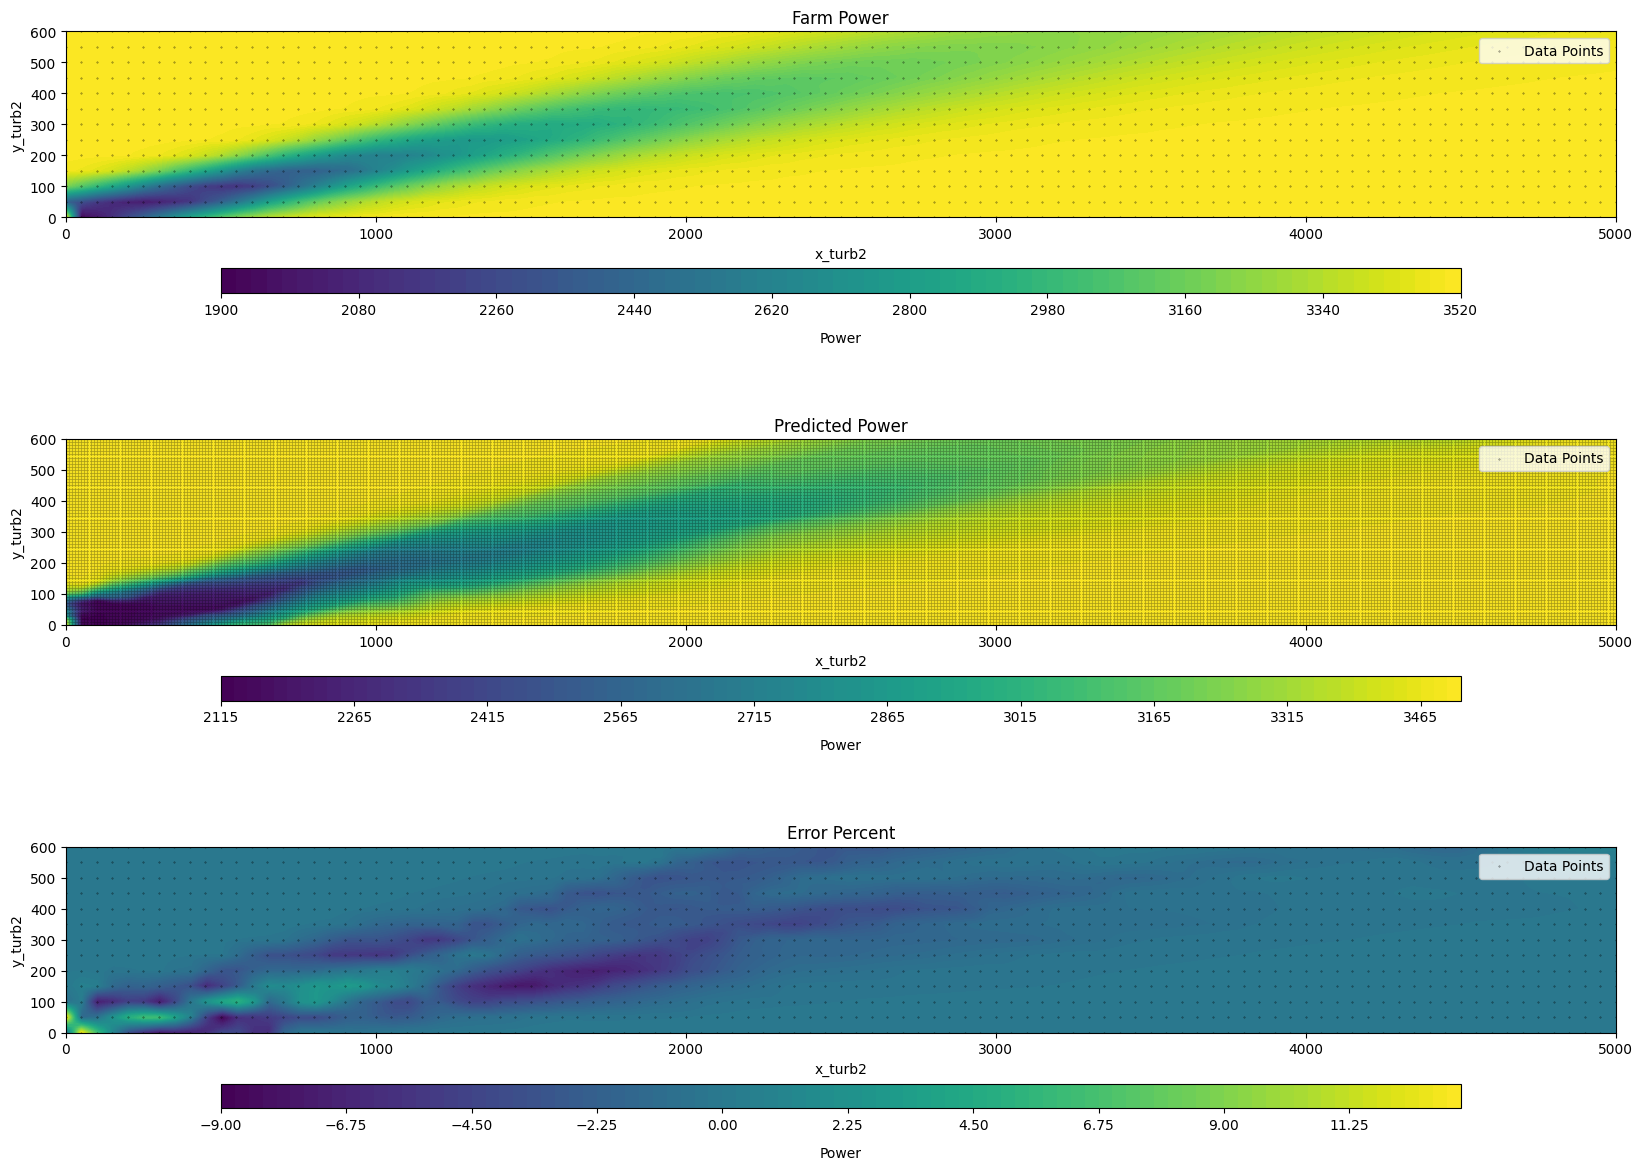
\includegraphics[width=1\textwidth]{figures/optimization/prob_model_colormap.png} 
	\caption{A heatmap of total generated farm power for a wind direction of 260° with datapoints and linear interpolation in between. Plot 1 shows the raw data, plot 2 the predictions of the $\text{NN}(5\,{-}\,50^{\times2}\,{-}\,1)$, plot 3 the percentage difference between training points and predictions}
	\label{fig:prob_model_colormap}
\end{figure}

Having observed the deviation described above, another layer is added to the model in an attempt to prevent the previous behaviour. The resulting configuration $\text{NN}(5\,{-}\,50^{\times3}\,{-}\,1)$ improved the previous models weaknesses in that respect as can be seen in Figure \ref{fig:prob_model_colormap_2}, which is why \textit{the final model choosen for the optimization is  $\text{NN}(5\,{-}\,50^{\times3}\,{-}\,1)$}

\begin{figure}[h] 
	\centering
	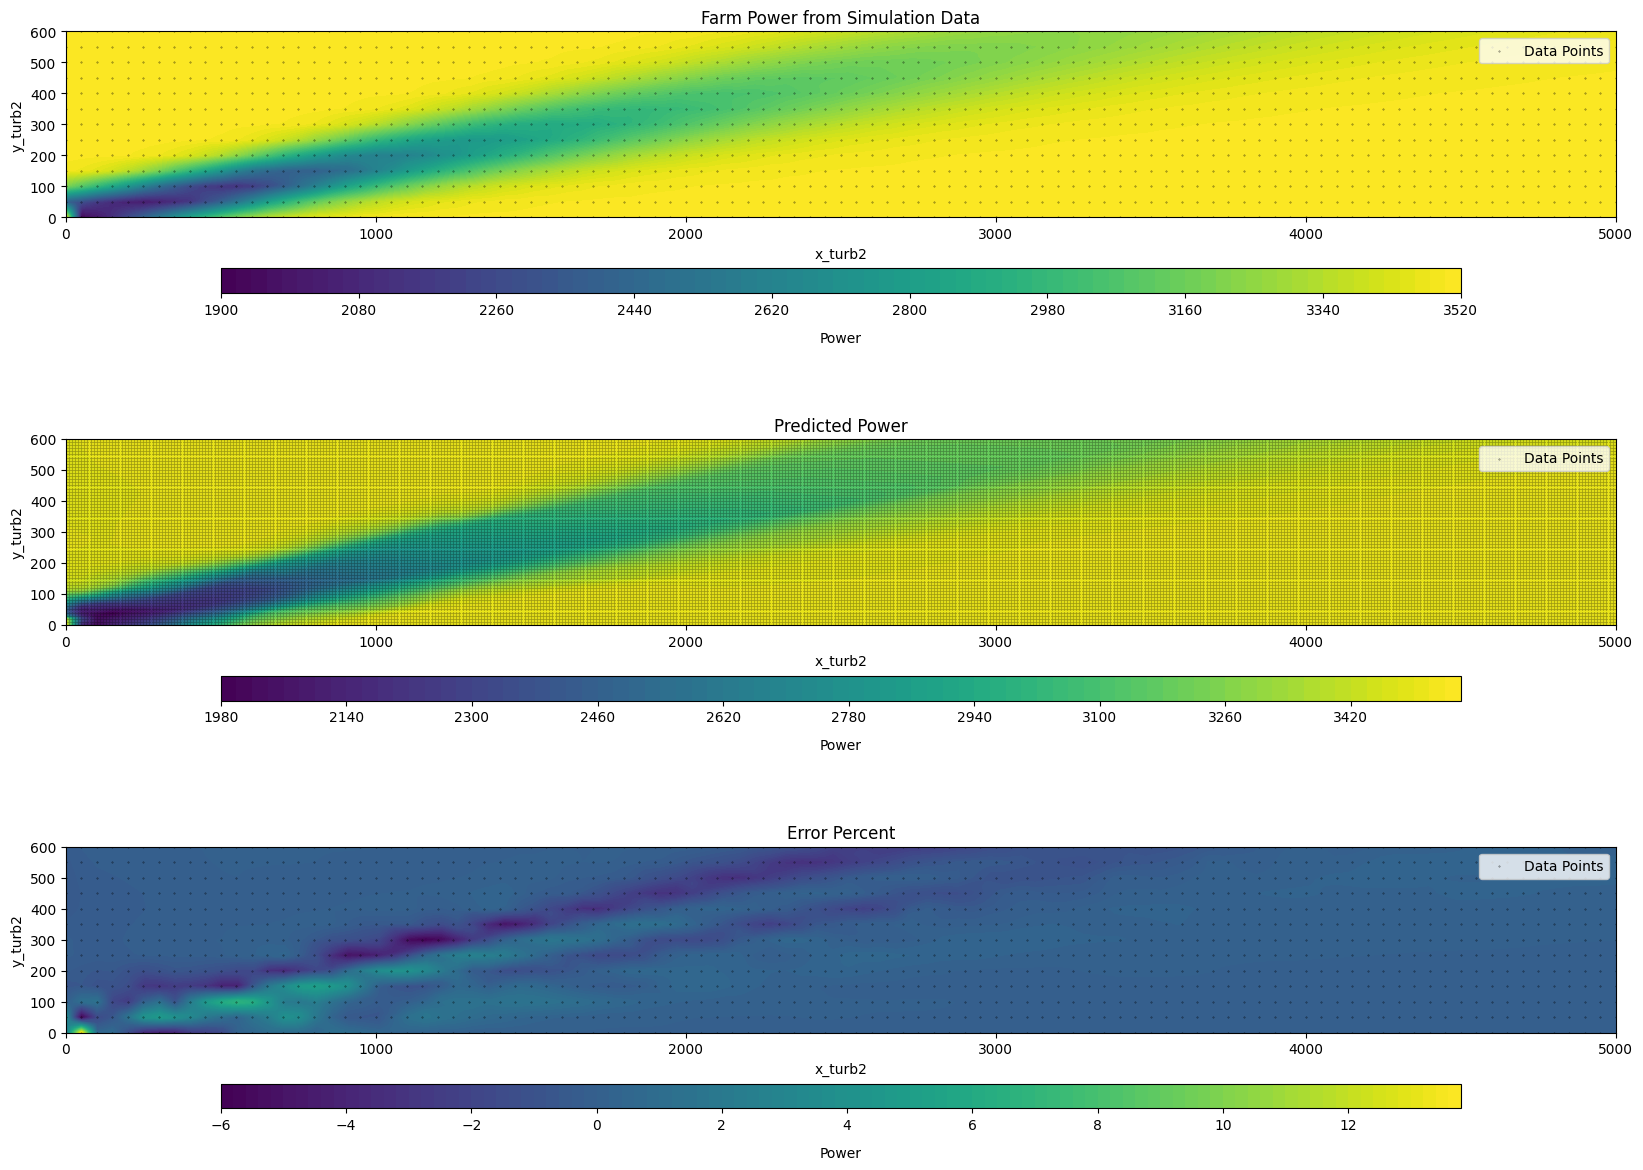
\includegraphics[width=1\textwidth]{figures/optimization/prob_model_colormap_2.png} 
	\caption{A heatmap of total generated farm power for a wind direction of 260° with datapoints and linear interpolation in between. Plot 1 shows the raw data, plot 2 the predictions of the $\text{NN}(5\,{-}\,50^{\times3}\,{-}\,1)$, plot 3 the percentage difference between training points and predictions, overall showing improved }
	\label{fig:prob_model_colormap_2}
\end{figure}

Since the parameter space has now become three-dimensional, conditioning on a single wind direction does not cover the full performance of the model. Figure \ref{fig:rmse_dist_3layers50nodes} shows the development of RMSE across different wind directions, indicating that the border regions and wind directions with an increased total wake length (e.g. wind directions closer to 270° wind direction) experience higher RMSE, providing more space for errors to accumulate. 

\begin{figure}[h!] 
	\centering
	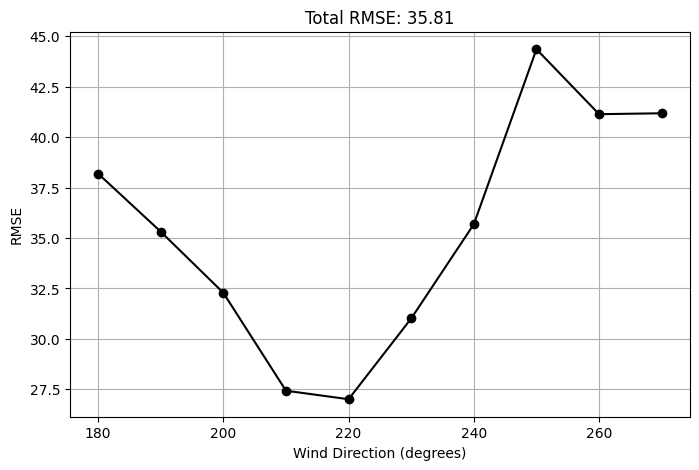
\includegraphics[width=0.55\textwidth]{figures/optimization/rmse_dist_3layers50nodes.png}
	\caption{RMSE of  $\text{NN}(5\,{-}\,25^{\times10}\,{-}\,1)$ across the parameter space of wind direction }
	\label{fig:rmse_dist_3layers50nodes}
\end{figure}

While increasing the size of the Neural Network might further reduce the deviations across wind directions and for the individual wind directions, it is restricted by the solvability of the optimization problem. While there is no exact threshold, the solving time of the mixed integer problem that results from the embedding of the Neural Network increases roughly exponentially by adding Neurons to the Network and therefore adding binary variables to the problem. The shown model is deemed sufficient because of that trade-off.

For optimization purposes, the individual power per wind direction becomes less relevant, as the power outputs are weighted by their probability of occurring. 
To do so, first the probability distribution of the wind directions has to be defined, like the Normal distribution with mean 270° and standard deviation of 10° shown in Figure \ref{fig:wind_dist_opti}. To calculate the expectation for the discretized parameter space using the trained model, this distribution itself has to be discretized in line with the initial parameter space defintion, which in this case is done in 10° steps. 


\begin{figure}[h] 
	\centering
	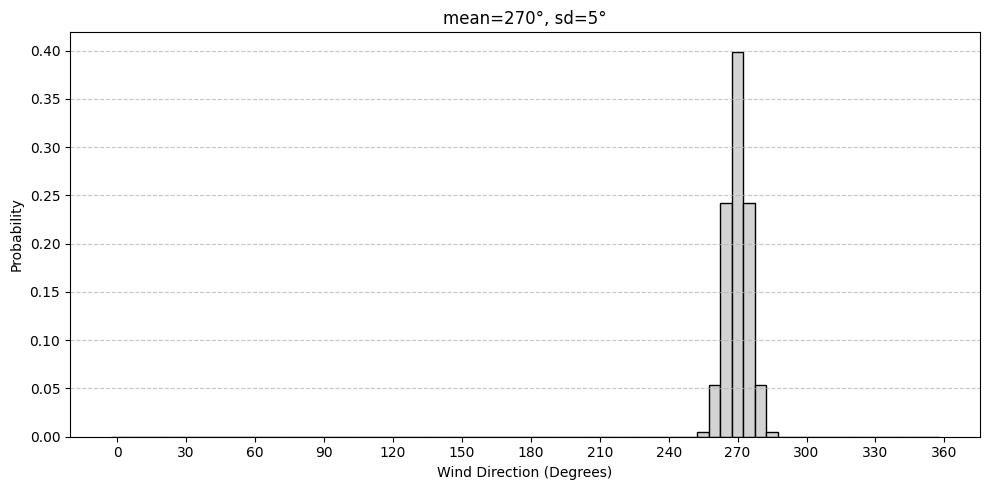
\includegraphics[width=1\textwidth]{figures/optimization/wind_dist_opti.png} 
	\caption{Discrete Wind Direction Probability Distribution with mean 270° and standard deviation 5°, discretized in intervals of 10° }
	\label{fig:wind_dist_opti}
\end{figure}


Using this distribution, the expected power for the ranges of x and y coordinates can thus now be calculated by aggregating the powers for the different wind directions as a sum weighted by probability to yield the expected farm power generated at the specific coordinate. By evaluating the expected farm power both for the training data as well as for predictions for the training data, we can again compare the results and deviations as done in Figure \ref{fig:prob_expectation}. The directions with a probability greater than are shown as lines and their impact on the distribution of expected farm power visibel.

\begin{figure}[h] 
	\centering
	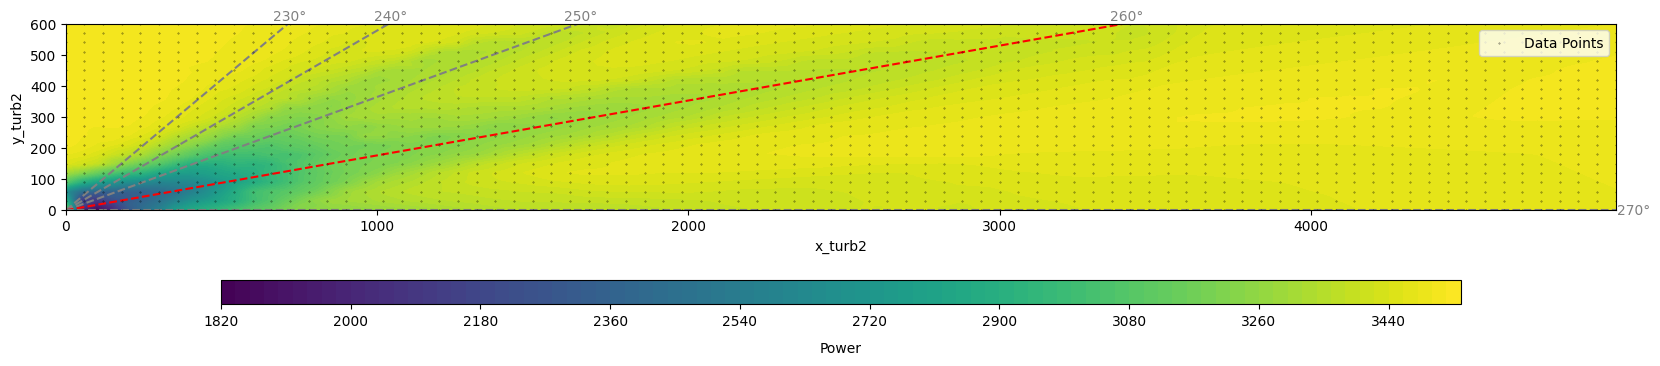
\includegraphics[width=1\textwidth]{figures/optimization/prob_expectation.png} 
	\caption{Distribution of Expectation of Farm power from a discretized Normal distribution with mean 260° and standard deviation 10° with steplength 10°}
	\label{fig:prob_expectation}
\end{figure}

In the same way the distribution of farm power was previously dependent on the deterministic wind direction, it is now dependent on the wind direction distribution, e.g. its mean and variance, assuming a Normal distribution. Changing the mean of the distribution corresponds to changing the direction of the principal wind direction and thus the direction of the highest expected wake losses from turbine 1. Meanwhile, increasing the variance corresponds to spreading the expected wake losses due to turbine 1 across a wider range of wind directions and therefore increasing the area affected by expected wake losses, while reducing the absolute reduction in expected power within the area affected by the wake. This relationship can be seen in the expected power distribution for a normal with mean 220° and standard deviation 20° shown in Figure \ref{fig:wind_dist_opti2}.


\begin{figure}[h!] 
	\centering
	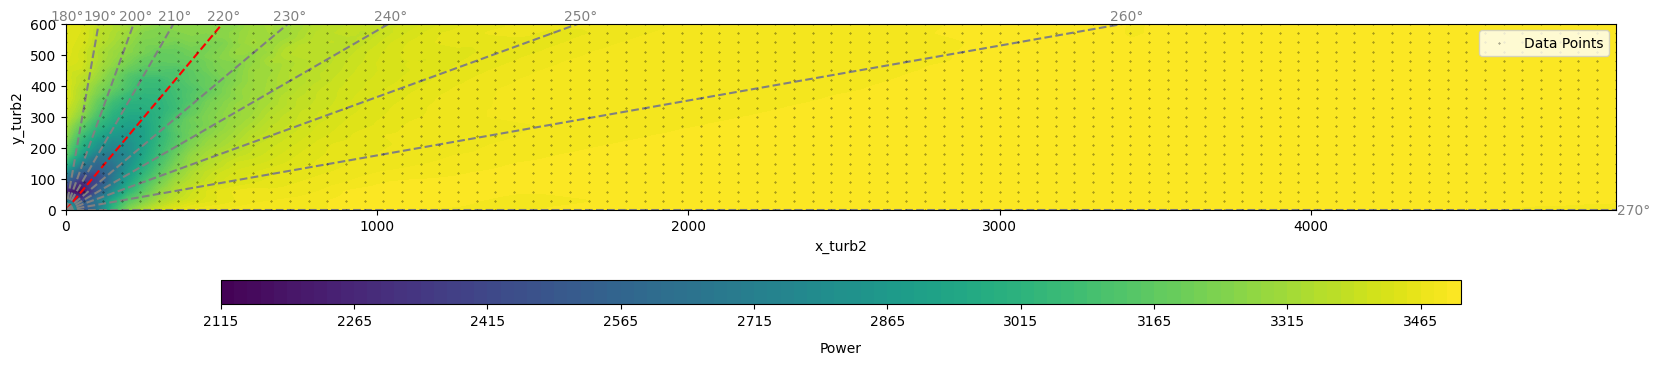
\includegraphics[width=1\textwidth]{figures/optimization/prob_expectation2.png} 
	\caption{Distribution of Expectation of Farm power from a discretized Normal distribution with mean 220° and standard deviation 20° with steplength 10°}
	\label{fig:wind_dist_opti2}
\end{figure}


The normal distribution is used in this thesis as a placeholder for proof-of-concept purposes. In a practical application, the real wind distribution would have to be evaluated at the specific location of the wind farm. 

\subsubsection{Optimization}

With the model set up, solving the stochastic optimization problem for a maximum expected farm power output can be attempted. In the case of optimization, the problem is limited to three scenarios due to the computational constraints due to the size of the problem. A normal distribution with a mean of 270° and  a standard deviation of 5° was therefore used as the wind direction distribution, yielding three scenarios (260°,270°,280°).

The Neural Network and the wind direction distribution are introduced into pyomo to find a global maximum. As previously, a range of optima exists, with Poyomo choosing among this area, as seen in Figure \ref{fig:prob_data_lininter}. More specifically in this case, the area close to the wake had been shown to predict higher values than in the simulations by the model (see Figure \ref{fig:prob_model_colormap_2}), showing the optimization to find the global maximum within the provided Neural Network. 

\begin{figure}[h] 
	\centering
	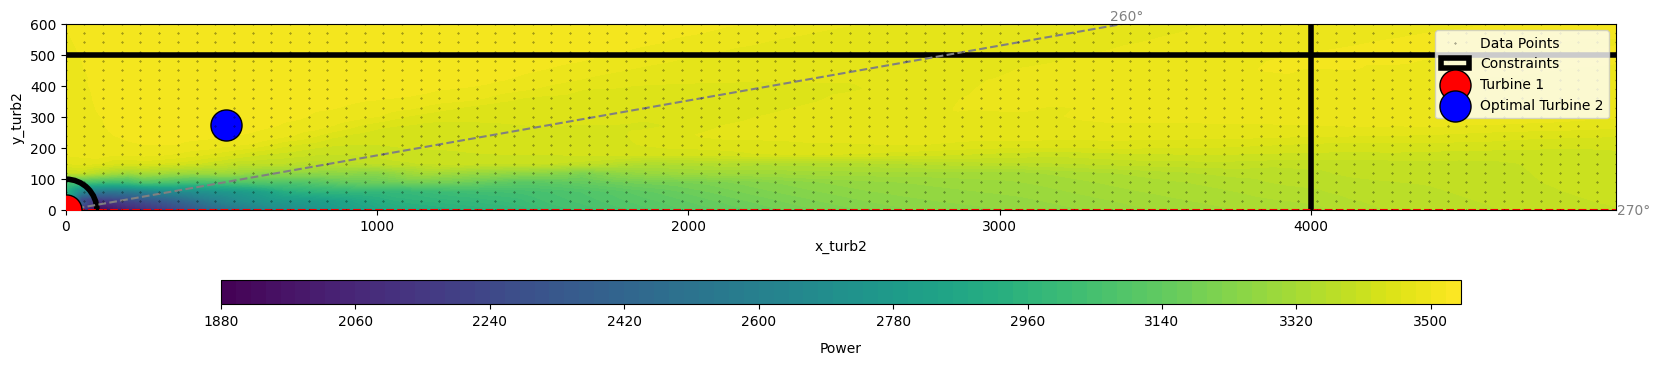
\includegraphics[width=1\textwidth]{figures/optimization/prob_data_lininter.png} 
	\caption{}
	\label{fig:prob_data_lininter}
\end{figure}

Like before, it is possible to visually find that there is a large range of more or less equally optimal points, with the few scenarios not covering the space appropriately. This leads to seemingly optimal areas in between the scenario wind directions, where in reality, significant wake losses can be expected. In addition to that, some small deviations of the model due to its complexity affect the optimization outcome significantly, with the current model predicting a maximum farm power production for turbine 2 placement close to the wake of turbine 1. Both of those aspects are weaknesses in the current configuration of the stochastic optimization.
	
\subsubsection{Stochastic Optimization: Quantile Discretization of Wind Direction Distribution } \label{subsubsection: discretization}

The first problem observed in this formulation as the gaps between the scenario wind directions as shown in Figure \ref{fig:prob_data_lininter}, can be partially solved by discretizing not with a constant step length but based on the quantiles of the distribution. The discretization can be instead performed not by a constant length of the discretization steps, but by a constant probability within a chosen number of quantiles. For each quantile individually, the mean is then calculated and the resulting expected values for the quantile are taken as discretization steps. This approach, when used for the same Normal distribution with mean 270° and standard deviation 5°, fixing the scenario/quantile count to 7, yields the discretization shown in Figure \ref{fig:wind_dist_opti_quantiles}. 

\begin{figure}[h] 
	\centering
	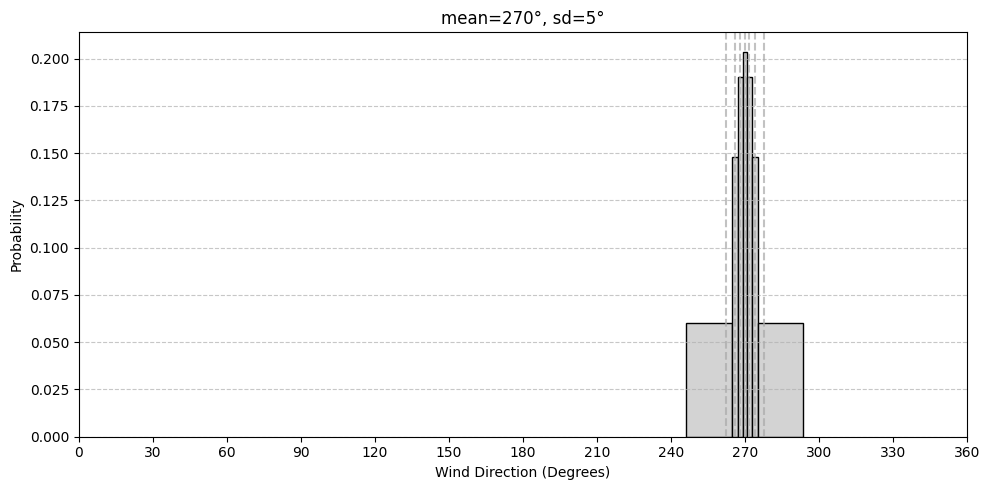
\includegraphics[width=0.8\textwidth]{figures/optimization/wind_dist_opti_quantiles.png} 
	\caption{Quantile based discretization of Normal mean 270°,  standard deviation 5°, disrcetized into 7 scenarios with equal probability for scenario and the scenario angle corresponding to the expected value for the quantile }
	\label{fig:wind_dist_opti_quantiles}
\end{figure} 

Using this distribution, the expected power distribution changes for the corresponding scenarios/quantiles, with the space left between scenarios proportional to the probability density. When considering the previous approach to stochastic optimization, the number of scenarios that can be introduced into the problem has now become the main limitation. The following subsection provides an alternative set up that allows for a greater number of scenarios.

\subsection{Stochastic Optimization: Direct Expectation Neural Network}

While the expectation maximization has shown to be the most accurate depiction of the problem on theoretical level, the previous method used for the resulting stochastic optimzation has shown to be severly limited by computational power, as a large Neural Network is required to model the farm power output both across x and y ranges of the second turbine, as well as across the wind condition variables. 
To overcome these constraints, a alternative formulation is set up, where the Neural Network is designed to output the expected farm power at any x/y point, given a certain wind condition distribution. 



\begin{align}
	\max_{\mathbf{x}, \mathbf{y}} &  \mathbb{E}[f_{Power}(\Delta x, \Delta y) \mid \text{wind condition distribution}]_\text{NN} \\
	\text{s.t.} \quad 
	&  0  \leq \Delta x \leq X_{\max} \\
	&  0  \leq \Delta y \leq Y_{\max} \\
	& \sqrt{(\Delta x)^2 + (\Delta y)^2} \geq d_{\min}
\end{align}

Where:
\begin{itemize}
	\item \( (\Delta x, \Delta y) \) are the relative distances of the two turbines,
	\item \( \mathbb{E}[f_{Power}(\Delta x, \Delta y) \mid \text{wind condition distribution}]_\text{NN}\) a Neural Network that predicts the Expected Farm Power at al \( (\Delta x, \Delta y) \) positions in the parameter space, given a specific wind speed distribution 
	\item \(  X_{\max}, Y_{\max} \) define the maximal distance the two turbines can be placed apart
	\item \( d_{\min} \) is the minimum distance between the two turbines
\end{itemize}

In practice, the new Neural Network configuration is achieved by training the Network directly on the Expected Farm Ppower Values, with the only remaining variables as the relative x/y position of the second wind turbine. To do so, the simulation values across the wind condition variables for a single location are used to calculate the expectation for that location as a probability weighted sum, with probabilities resulting from the distribution of the wind condition variables (wind direction, etc). To combine this approach with quantile discretization from Section \ref{subsubsection: discretization}, the resulting quantile scenario discretization is used to define the parameter space for the initial data set generating simulations. That way, a match between the scenario values and data set discretizations can be assured to allow for seemless calculation of the expectations. 

The central benefit of this formulation is that the dimensionality of the Neural Network is significantly reduced, with only  \(\Delta x, \Delta y\) remaining free after calculating the expectations. The drawback ist that the model is thus condition on a spcific wind condition distribution and can not be used in a more flexible way.


The Notebook belonging to this formulation can be found in \href{https://github.com/schmeti/uc3m_TFM_wind_farm_optimization_codebase/blob/main/Windfarm_power_modelling/0_two_turbine_problem_constrLearn_probweightedt_expNN.ipynb}{Stochastic optimization with farm power Expectation NN Fomulation Notebook} \cite{schmetz2025twoturbine_stoch2}

\subsubsection{Modelling}

To generate the model with the farm power expectation as output, more steps are required as initially described in Chapter \ref{sec:model_pipe}. As detailed in the introduction, for the configuration used in this chapter, the Wind Condition distribution, which in this case will only be the distribution of wind directions, has to be defined. For this wind distribution, a discretization is generated the quantile based method described in Section \ref{subsubsection: discretization}. From this discretization, together with chosen limits for \(\Delta x, \Delta y\), the parameter grid/space is defined and corresponding simulation performed to generate the data set. The probabilities from the wind condition distribution are then joined to the dataset and used to calculate the Expected Farm power for each \(\Delta x, \Delta y\) combination in the parameter grid. This yields a significantly smaller data set with \(\Delta x, \Delta y\) and Expected Farm power as features. This dataset is then used to train a model in the same way done previously, choosing a appropriat configuration of the model which then is used for embedding in the optimization problem. The described steps are shown in Figure \ref{fig:stoch2_model_flow}.


\begin{figure}[h] 
	\centering
	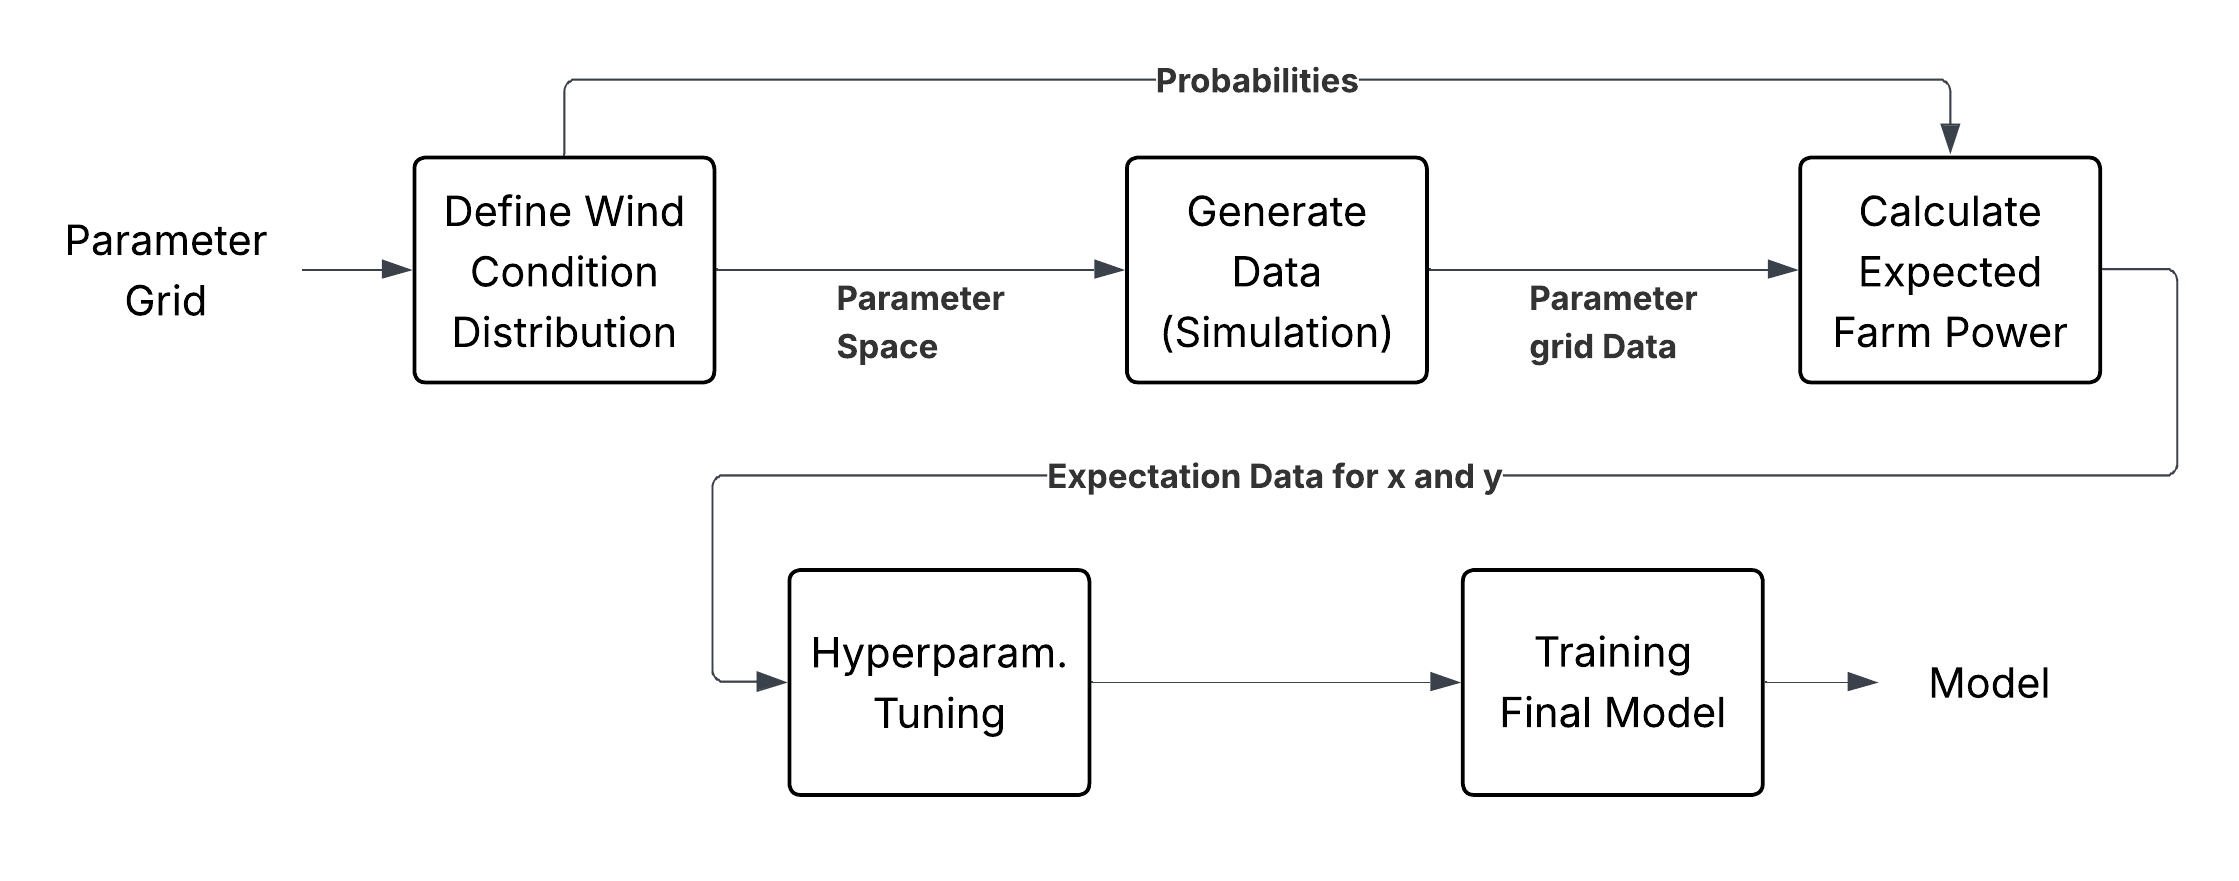
\includegraphics[width=1\textwidth]{figures/optimization/stoch2/stoch2_model_flow.png} 
	\caption{Flowchart displaying the steps used to set up a Neural Network model to model Expected Farm Power across \(\Delta x\) and  \(\Delta y\)}
	\label{fig:stoch2_model_flow}
\end{figure} 

As previously, we proceed to defining the parameter space, with the only difference compared to the previous stochastic formulation is that the wind direction how has variable steplength, using the method presented in Section \ref{subsubsection: discretization}.

\begin{table}[ht]
	\centering
	\caption{Value Ranges for Stochastic Expectation Neural Network Two Turbine Problem Data Set}
	\begin{tabular}{|l|c|c|c|}
		\hline
		\textbf{Variable} & \textbf{Const/Variable} & \textbf{Value} & \textbf{$Steplength$}\\
		\hline
		$\Delta x_{\text{turb2}}$ & Variable & [0, 5000] m & 50 m\\
		$\Delta y_{\text{turb2}}$ & Variable & [0, 500] m  & 50 m\\
		wind\_speed & Constant & 8 m/s & -\\
		wind\_direction & Variable & [180°, 270°]& 35 Quantiles \\
		turbulence\_intensity & Constant & 0.06 & - \\
		\hline
	\end{tabular}
	\label{tab:val_prob2_data}
\end{table}

As at this stage the parameter grid for wind direction is not yet well defined, the wind direction distribution and the number of discretization steps first has to be chosen. For this section, we proceed with the same normal distribution mith mean 260° and standard deviation 10° used in Section \ref{sec:stoch_opti_1}, but now discretized for 35 quantiles as shwon in Figure \ref{fig:stoch2_dist}.


\begin{figure}[h] 
	\centering
	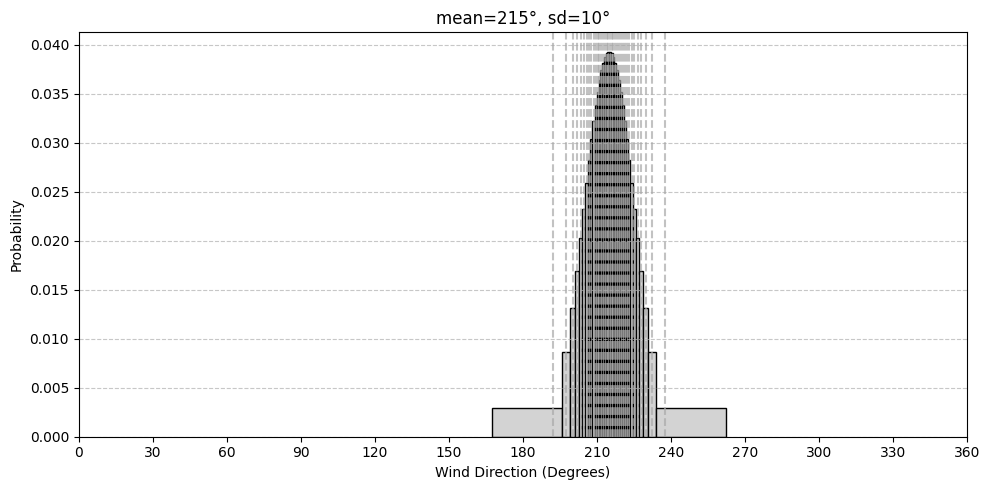
\includegraphics[width=0.8\textwidth]{figures/optimization/stoch2/dist_discret.png} 
	\caption{Quantile based discretized Normal with mean 260° and standard deviation 10°, discretized for 35 quantiles}
	\label{fig:stoch2_dist}
\end{figure} 

With the parameter grid defined, the simulations can be performed, joint with the wind condition probabilities and expectations for the farm power calculated, yielding the dataset to be used in the training of the Neural Network. We thus proceed to the grid search optimization of the Neural Network configuration, as done in the previous chapters. For the distribution shown above, we find the 2-hidden layer and 20 neurons per hidden layer $\text{NN}(5\,{-}\,20^{\times2}\,{-}\,1)$ configuration to yield the best results for least numbers of neurons, as can be seen in Figure \ref{fig:stoch2_NNopti}. \textit{We thus proceed with the configuration $\text{NN}(5\,{-}\,20^{\times2}\,{-}\,1)$}.


\begin{figure}[h] 
	\centering
	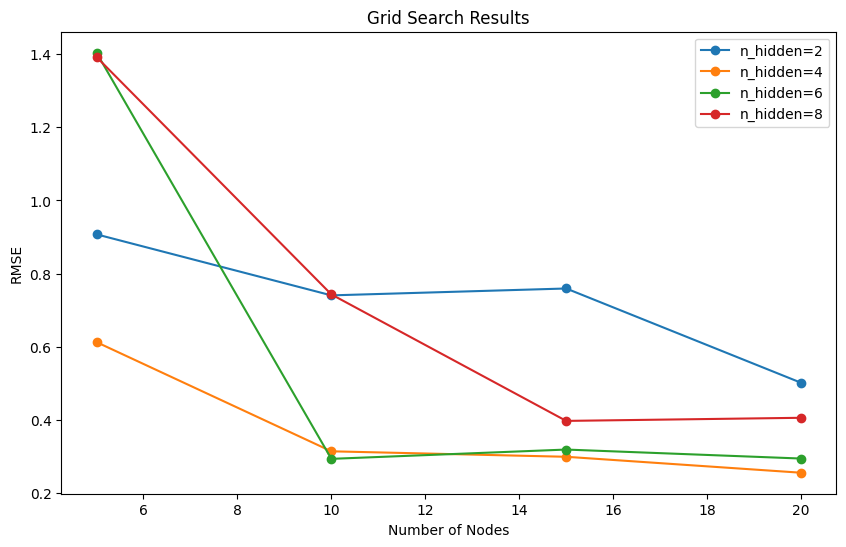
\includegraphics[width=0.8\textwidth]{figures/optimization/stoch2/stoch2_NNopti.png} 
	\caption{Grid Search Results for models trained on Farm Power Expectation data, with parameter grid as defined in Table 	\ref{tab:val_prob2_data} and Figure  \ref{fig:stoch2_dist} }
	\label{fig:stoch2_NNopti}
\end{figure} 


The model of configuration $\text{NN}(5\,{-}\,20^{\times2}\,{-}\,1)$ is thus trained and a brief visual inspection performed to investigate how well the model fits the data. As shown in Figure \ref{fig:stoch2_heatmap_inspect_NN}, does the model encorporate the shape of the Expected Power Distribution across x/y fairly well, with the only major deviations near the orgin, e.g. the position of Turbine 1 and directly after Turbine 1 in the principal wind direction. 

\begin{figure}[H] 
	\centering
	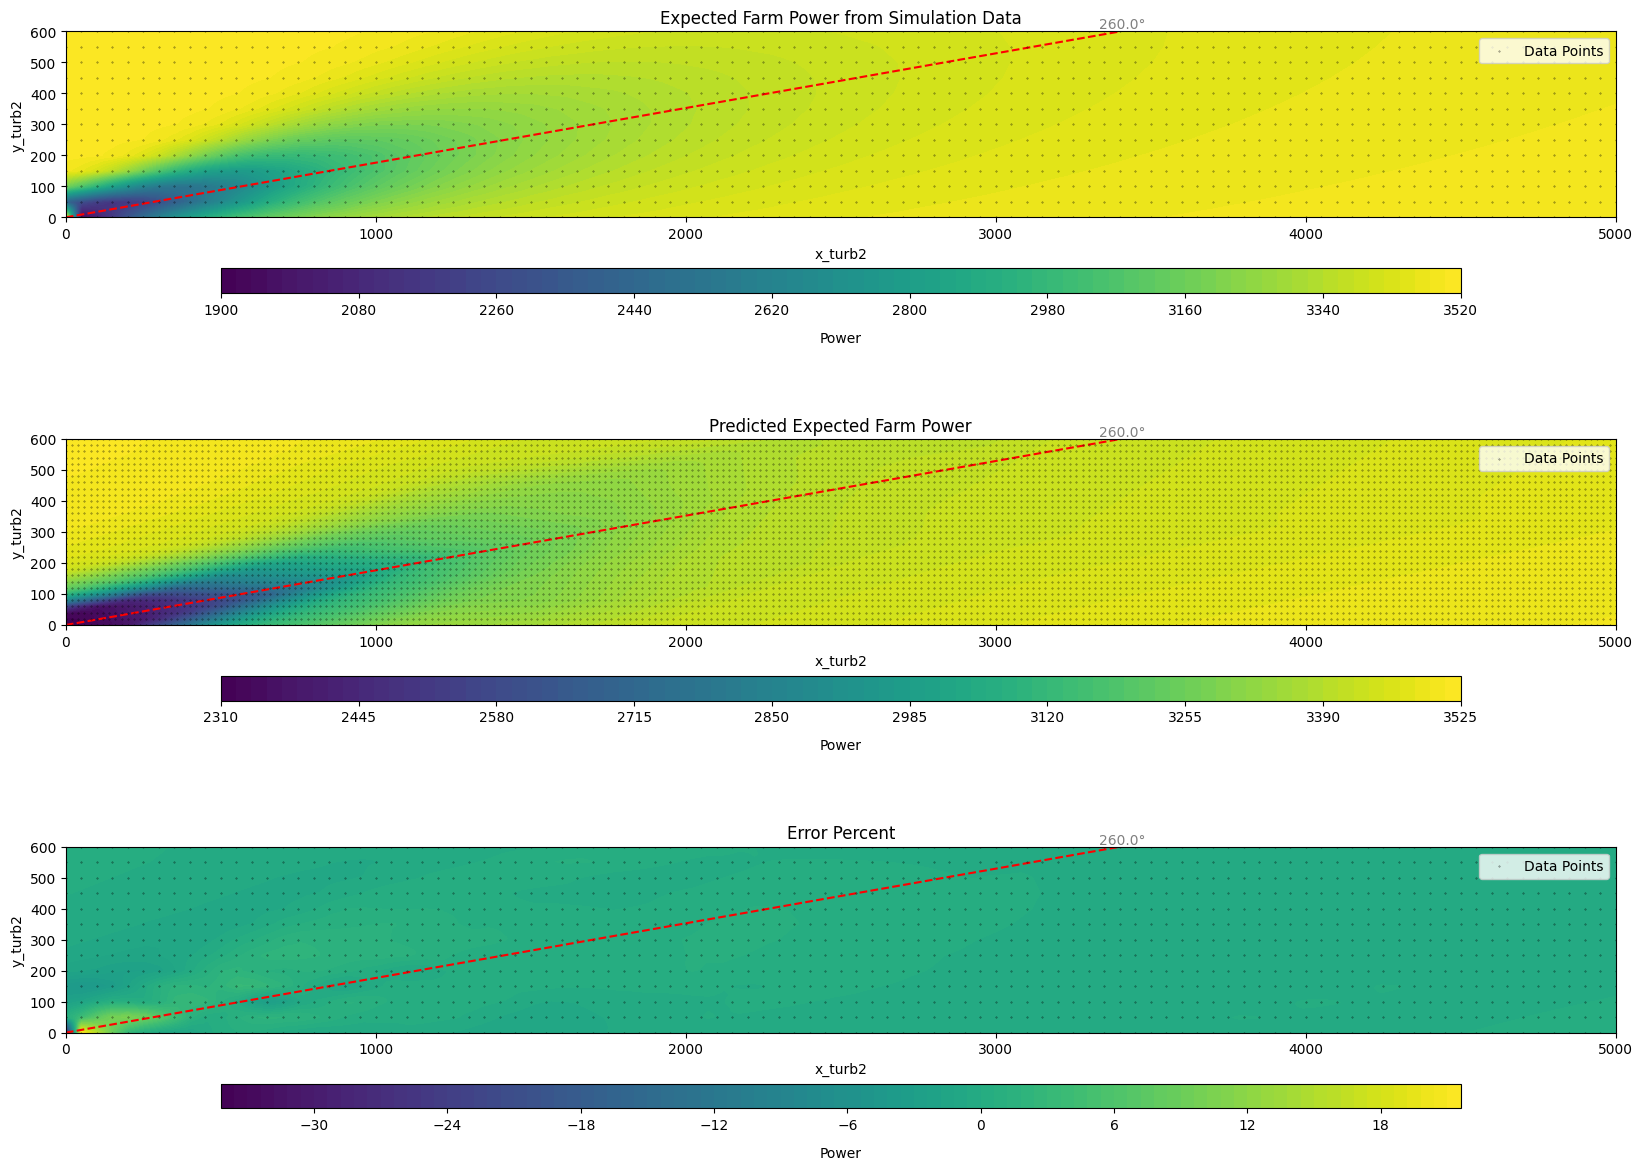
\includegraphics[width=1\textwidth]{figures/optimization/stoch2/stoch2_heatmap_inspect_NN.png} 
	\caption{Visual comparison of training data vs predictions for Neural Network for Expectation of Farm Power, with linear interpolation in between data points to generate heatmap}
	\label{fig:stoch2_heatmap_inspect_NN}
\end{figure} 

The model thus appears to fit the physical behavior suficiently well to be able to proceed to the optimization step. 



\subsubsection{Optimization}

The set up model is thus again embedded into a now seemingly deterministic optimization problem, as the uncertainty has already been taken into account when setting up the Neural Network itself through the expectations. The Neural Network is thus embedded directly into the problem, with the constraints as initially defined. The result shown in Figure \ref{fig:stoch2_opti} yield the expected result, with turbine 2 being placed as far upstream and as far away perpendicularly to the principal wind direction as possible from Wind Turbine 2. 

\begin{figure}[h] 
	\centering
	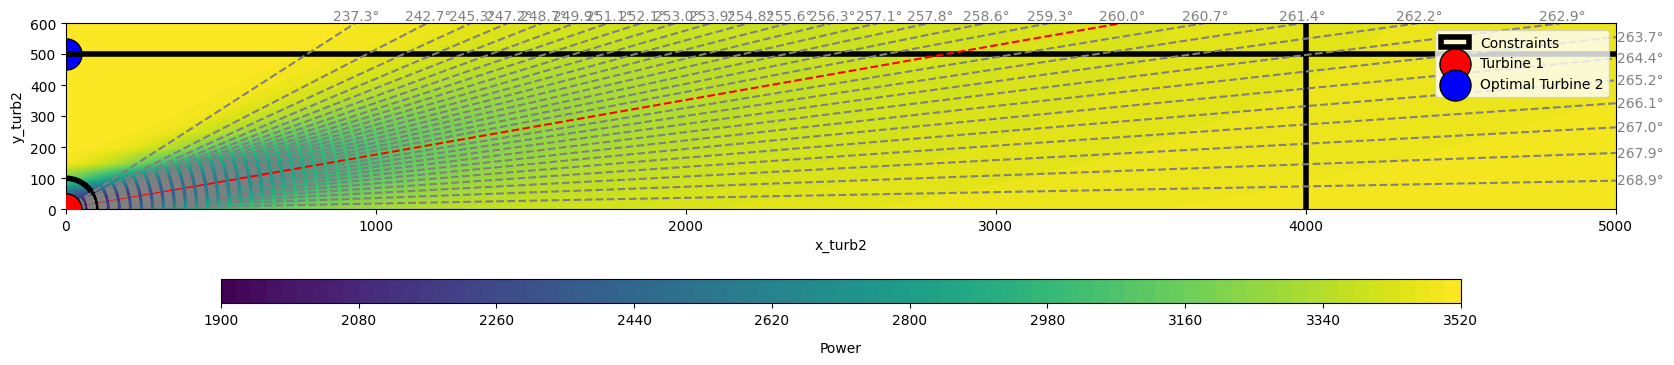
\includegraphics[width=1\textwidth]{figures/optimization/stoch2/stoch2_opti.png} 
	\caption{Optimization Result for maximization of Expected Farm Power, with wind direction Normally distributed with mean 260° and standard deviation 10°, discretized into 35 scenarios using quantile based discretization and Neural Network configuration $\text{NN}(5\,{-}\,20^{\times2}\,{-}\,1)$ }
	\label{fig:stoch2_opti}
\end{figure} 

Notably, the solving of this variation optimization problem requires significantly less computational recourses as the previous stochastic formulation, with a significantly larger quantity of scenarios considered for calculating the Expectation. In the entire optimization pipeline, the main limitation is in this formulation constitued by running the simulations required for the individual discretization of different wind direction/wind condition distributions. Due to the efficency of the FLORIS simulations, this does not seem to be a limitation for the two turbine configuration at this moment however. Therefore, this method appears to be better fit to scale up the complexity of the wind condition distribution, allowing for expanding to a multivariate distribution of the potentially dependent variables wind direction and wind speed for example. 

%\subsection{Thoughts}
%
%IDEA: Use big neural Network to replace simulations
%
%IDEA: generalize inputs in a way that allow for power calculation of each turbine individually instead of farm power
%
%IDEA : derive basic rules from 2 turbine problem and set up new optimization problem without NN 
%
%IDEA : analogue to forward/backward selection with 2 turbine neural network
%
%
%FINIDINGS: 
%
%problem degenerate if not one wind turbine fixed

